\chapter{Data Driven Classification of P Cygni and Inverse P Cygni Spectra}

\section{A Framework for Classification}

It is clear from the prior chapter that a classification approach to P Cygni and inverse P Cygni spectra must follow a morphology based scheme. While morphological classification based on naked eye observations of spectra has been used in the past, this approach cannot scale with the volume of data present in million star sky surveys and certainly cannot scale effectively on DR3. In terms of automated methods that can scale more effectively, approaches such as t-SNE and autoencoders \cite{traven2017galah,vcotar2021galah} have been successful in detecting H$\alpha$ emission spectra. While the former was not able to reliably identify a broader sample of these candidate spectra, the latter was able to identify several thousand potential H$\alpha$ spectra in DR3 using an anomaly detection approach (autoencoders). These recent methods, and notably latter have shown the greatest success in identifying H$\alpha$ candidates in DR3. However they fall short in the automated identification of P Cygni and inverse P Cygni spectra in DR3.

Given that DR3 does not have suitable labeled samples of P Cygni and inverse P Cygni spectra, a supervised learning approach to classification is not suitable. This narrows the field of possible technical and scientific approaches to the unsupervised classification domain \cite{hastie2009elements}. A classification approach that is sensitive to the meaningful morphological differences between P Cygni and inverse P Cygni also remains an important requirement. Feature engineering tasks that need to be performed to prepare the raw data must take into account the understanding that P Cygni spectra exhibit a red shifted emission peak while the inverse P Cygni spectra exhibit a blue shifted peak. Finally, given that the feature space is $\approx$ \num[round-precision=2,round-mode=figures, scientific-notation=true]{2928752091}, the classification approach must be able to grapple with this dimensionality and overcome the "curse of dimensionality".

\section{Time Series Clustering}

A full treatment of unsupervised clustering and classification methods is beyond the scope of this work, however this section will briefly introduce time series clustering, more specifically unsupervised time series clustering. It was noted in a prior chapter that DR3 spectra and indeed all spectra can be modeled as "time series". While an individual spectrum does not contain a time axis, the monotonically increasing wavelength grid serves as the analogue of the time axis in the context of traditional numerical computing methods. These machine learning methods have been more generally developed in the domain of time series analysis \cite{nielsen2019practical} and can be suitably adapted to stellar spectra. With clustering, we do not rely on labelled data, but rather develop a suitable method to cluster similar spectra into groups. Similar in this context being morphologically similar spectra such as P Cygni and inverse P Cygni.

\subsection{Dynamic Time Warping}

Dynamic time warping (DTW) is a time series analysis algorithm that can measure similarity between two temporal sequences. The similarity can then be used to cluster similar spectra into meaningful groups. These clusters can then be used to classify spectra into distinct classes. DTW is suitable for clustering problems where the morphology of the signal plays a salient role \cite{nielsen2019practical}. The name of the algorithm itself is inspired by the methodology where two signals are warped to align them on the temporal domain. For stellar spectra, this warping takes place in the wavelength domain. 

\begin{figure}[h]
\centering
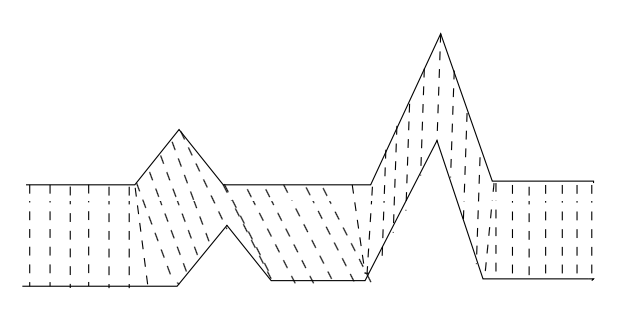
\includegraphics[scale=0.90]{figures/Dynamic_time_warping.png}
\caption{Each point on the wavelength grid is mapped to a point on the opposite spectrum, but there is no requirement that the mapping is one to one. Reproduced from Nielsen \cite{nielsen2019practical}}
\end{figure}

As indicated in the figure above, expansion or contraction of the wavelength axis to find the best alignment ensures that the shape of the spectra (the morphology) play a dominant role in determining similarity. This algorithm is often described as being akin to comparing the visual "shape" of the spectra, rather than focusing on the sequence of how these shapes are formed on the wavelength axis. The implications of this will be discussed in detail in this chapter. The algorithm follows a number of constraints which are,

\begin{enumerate}
    \item Every point on the spectrum must be matched with at least one point of the other spectrum
    \item The first and last indices of each spectrum must be matched with their counterparts in the other spectrum
    \item The mapping must be such that the wavelength is increasing rather than decreasing i.e. do not match a point on on spectrum to a point on the other spectrum that has "passed"
\end{enumerate}

Points 2 and 3 above do not have a significant impact on the DR3 dataset being used in this research as they are sampled to the same wavelength and thus are of equal length. There are many possible ways to align two spectra while adhering to these constraints. However the algorithm chooses the match 

